\documentclass[11pt,a4paper]{article}

\usepackage[brazil]{babel}
\usepackage[T1]{fontenc}
\usepackage{lmodern}
\usepackage{microtype}
\usepackage[margin=2.2cm]{geometry}
\usepackage{amsmath}
\usepackage{booktabs}
\usepackage{tabularx}
\usepackage{enumitem}
\usepackage{graphicx}
\usepackage{float}
\usepackage{caption}
\usepackage[hidelinks]{hyperref}

\setlist{nosep, leftmargin=*}
\setlength{\parskip}{0.4em}
\setlength{\parindent}{0pt}
\captionsetup{font=small, labelfont=bf}
\graphicspath{{figuras/}}

\title{\textbf{Q-learning nos ambientes Toy Text do Gymnasium}\\[0.3em]
  \large Relatório de experimentos}
\author{Caio Trindade\\
  \small Inteligência Artificial para Jogos I --- Aprendizado por Reforço}
\date{Novembro de 2026}

\begin{document}
\maketitle

\textbf{Código:} o notebook com a implementação, os experimentos e todas as saídas é o arquivo
\texttt{qlearning\_toy\_text.ipynb}, disponível em:\\
\url{https://github.com/ctrindadedev/game-ai-lab/tree/master/QLearningToyText}

O objetivo foi experimentar o Q-learning tabular no Lago Congelado, partindo do notebook disponibilizado na
disciplina, variar seus hiperparâmetros e testá-lo em outros ambientes do Toy Text. O agente é o mesmo do notebook
original: uma Q-table atualizada por diferença temporal,
\[
Q(s,a) \leftarrow Q(s,a) + \alpha\left[r + \gamma \max_{a'} Q(s',a') - Q(s,a)\right],
\]
com política $\varepsilon$-greedy e decaimento linear de $\varepsilon$. Quando o episódio termina (\texttt{terminated}),
o alvo é apenas $r$; quando é truncado pelo limite de passos, o alvo continua usando $\max_{a'} Q(s',a')$.

\section{Ambientes}

\subsection*{FrozenLake-v1 (Lago Congelado)}

\begin{itemize}
  \item \textbf{Estados:} a célula do grid, $\text{linha} \times n_{\text{colunas}} + \text{coluna}$: 16 no mapa 4x4
    e 64 no 8x8.
  \item \textbf{Ações:} 4 (esquerda, baixo, direita, cima).
  \item \textbf{Reforço:} $+1$ ao chegar no objetivo \texttt{G} e $0$ em qualquer outro passo, inclusive ao cair num
    buraco \texttt{H}, que encerra o episódio. O limite é de 100 passos.
  \item \textbf{Escorregadio} (\texttt{is\_slippery=True}): o agente só vai na direção escolhida com probabilidade
    $1/3$; nas outras vezes desliza para uma das direções perpendiculares.
  \item \textbf{Desafios:} a recompensa é esparsa. Até o agente chegar ao objetivo por acaso, a Q-table fica toda
    zerada e ele anda aleatoriamente. No gelo escorregadio, a mesma ação pode levar a estados diferentes, então os
    valores Q passam a estimar uma média de resultados aleatórios e nem a política ótima ganha sempre.
\end{itemize}

Foram usados dois mapas. O 8x8 é gerado como no notebook original
(\texttt{generate\_random\_map(size=8, p=0.9)}), mas com semente fixa (9), escolhida por ser de dificuldade
intermediária entre os dez mapas do Experimento 1. Ele tem 9 buracos. O 4x4 é o mapa padrão do Gymnasium, com 4
buracos. A melhor taxa de sucesso possível no gelo escorregadio, calculada por iteração de valor sobre o modelo do
próprio ambiente com horizonte de 100 passos, é \textbf{0,744} no 4x4 e \textbf{0,892} no 8x8. Esses valores servem de
teto para comparar os resultados do Q-learning.

\begin{center}
\footnotesize
\renewcommand{\arraystretch}{0.8}
\begin{tabular}{cc}
\texttt{SFFFFHFH} & \texttt{SFFF}\\
\texttt{FFFFFFHF} & \texttt{FHFH}\\
\texttt{FFFFFFHH} & \texttt{FFFH}\\
\texttt{FHFFHFFF} & \texttt{HFFG}\\
\texttt{FFFFFHFF} & \\
\texttt{FFFFHFFF} & \\
\texttt{FFFFFFFF} & \\
\texttt{FFFFFFFG} & \\[0.3em]
8x8 (semente 9) & 4x4 (padrão)
\end{tabular}
\end{center}

\subsection*{CliffWalking-v1 (Caminhada no Penhasco)}

\begin{itemize}
  \item \textbf{Estados:} 48 (grid 4x12). O início fica no canto inferior esquerdo e o objetivo, no inferior direito.
  \item \textbf{Ações:} 4 (cima, direita, baixo, esquerda).
  \item \textbf{Reforço:} $-1$ por passo e $-100$ ao pisar no penhasco (as 10 células entre o início e o objetivo),
    o que manda o agente de volta ao início sem encerrar o episódio. O retorno ótimo é $-13$.
  \item \textbf{Desafios:} o caminho mais curto passa colado no penhasco, então qualquer passo exploratório ali custa
    $-100$. O ambiente não tem limite de passos; usamos 200, porque sem limite uma política gulosa que anda em
    círculos nunca terminaria a avaliação.
\end{itemize}

\subsection*{Taxi-v4 (Táxi)}

\begin{itemize}
  \item \textbf{Estados:} 500 (25 posições do táxi $\times$ 5 posições do passageiro $\times$ 4 destinos).
  \item \textbf{Ações:} 6 (sul, norte, leste, oeste, pegar, deixar).
  \item \textbf{Reforço:} $-1$ por passo, $+20$ ao entregar o passageiro no destino e $-10$ ao tentar pegar ou deixar
    no lugar errado. O limite é de 200 passos. O retorno ótimo médio é 8,46, e o Gymnasium considera o ambiente
    resolvido a partir de 8.
  \item \textbf{Desafios:} o espaço de estados é bem maior e a tarefa tem duas etapas (buscar e entregar).
\end{itemize}

\section{Metodologia experimental}

\subsection{Configuração dos experimentos}

A configuração base é a do notebook original, e cada experimento muda um parâmetro por vez:

\begin{center}
\small
\begin{tabular}{ll}
\toprule
Parâmetro & Valor base \\
\midrule
Taxa de aprendizado $\alpha$ & 0,5 \\
Fator de desconto $\gamma$ & 0,95 \\
$\varepsilon$ ($\varepsilon$-greedy) & de 0,5 até 0,1, decaimento linear ao longo do treino \\
Episódios de treino & 5000 \\
Repetições & 5 sementes (0 a 4) por configuração \\
\bottomrule
\end{tabular}
\end{center}

\begin{itemize}
  \item \textbf{Experimento 0:} configuração base no FrozenLake 8x8 determinístico.
  \item \textbf{Experimento 1:} a configuração base em 10 mapas 8x8 aleatórios (sementes 0 a 9), com 3 sementes do
    agente em cada um, para medir o quanto o resultado depende do mapa.
  \item \textbf{Experimento 2:} variação de $\alpha \in \{0{,}01;\ 0{,}1;\ 0{,}5;\ 0{,}9\}$,
    $\gamma \in \{0{,}5;\ 0{,}9;\ 0{,}95;\ 0{,}99\}$, $\varepsilon$ inicial $\in \{0{,}1;\ 0{,}5;\ 1{,}0\}$ e
    $\varepsilon$ final $\in \{0{,}01;\ 0{,}1;\ 0{,}3\}$, no 8x8 determinístico e no 4x4 escorregadio.
  \item \textbf{Experimento 3:} tamanho do mapa (4x4 e 8x8) e gelo escorregadio. O 8x8 escorregadio também foi
    treinado com 20000 episódios, com $\alpha = 0{,}5$ e com $\alpha = 0{,}1$.
  \item \textbf{Experimento 4:} CliffWalking-v1 e Taxi-v4 com a configuração base.
\end{itemize}

\textbf{Hipóteses iniciais.}
(H1) No ambiente determinístico, os hiperparâmetros devem afetar mais a velocidade do que a política final.
(H2) No escorregadio, um $\alpha$ alto deve atrapalhar, porque cada resultado aleatório altera muito a Q-table.
(H3) Um $\gamma$ baixo deve atrapalhar em caminhos longos com recompensa só no fim.
(H4) Um $\varepsilon$ final maior deve piorar a recompensa durante o treino.
(H5) No CliffWalking, a política aprendida deve ser a ótima (colada no penhasco), mas o retorno de treino deve
ficar bem abaixo dela por causa da exploração.

\textbf{Critério de parada:} número fixo de episódios. Cada episódio termina num estado terminal ou no limite de
passos. \textbf{Ferramentas:} Python 3.12, Gymnasium 1.4, NumPy, pandas, Matplotlib e seaborn, em um notebook Jupyter
que também roda no Colab.

Em relação ao notebook original, o mapa foi fixado, cada configuração foi repetida com várias sementes e a política
gulosa passou a ser testada a cada 25 episódios em vez de 100 (com 100, quase tudo já tinha convergido na primeira
avaliação). Também foram removidos os imports do pacote antigo \texttt{gym} e a gravação de vídeos.

\subsection{Procedimentos de treinamento e avaliação}

Em cada episódio de treino, o agente escolhe ações com $\varepsilon$-greedy e atualiza a Q-table a cada passo. Ao
fim do episódio, $\varepsilon$ diminui linearmente. O desempenho foi medido de três formas:

\begin{itemize}
  \item \textbf{Recompensa de treino:} recompensa total por episódio (no FrozenLake, 1 em caso de sucesso), em média
    móvel de 100 episódios. Reflete o aprendizado, mas inclui os erros da exploração.
  \item \textbf{Teste guloso:} a cada 25 episódios, a política gulosa ($\varepsilon = 0$, sem atualizar a tabela)
    joga 20 episódios. Ao fim do treino, joga mais 500 episódios para a \textbf{avaliação final}. No FrozenLake isso
    é a taxa de sucesso; nos outros ambientes, o retorno médio.
  \item \textbf{Convergência:} o primeiro episódio em que o teste guloso atinge um limiar (90\% de sucesso no
    FrozenLake determinístico, 70\% no escorregadio e o retorno ótimo nos outros ambientes).
\end{itemize}

As curvas mostram a média entre as 5 sementes, com faixa de $\pm 1$ desvio padrão, que indica a estabilidade. As
tabelas trazem média e desvio padrão entre as sementes. A política aprendida é visualizada como um mapa de calor do
maior valor Q de cada estado, com uma seta para a melhor ação.

\section{Resultados}

\subsection*{Configuração base e efeito do mapa}

No 8x8 determinístico, a configuração base atingiu 100\% de sucesso guloso em todas as sementes, com 90\% de sucesso
pela primeira vez por volta do episódio $855 \pm 173$. A recompensa de treino nos últimos 500 episódios foi
$0{,}896 \pm 0{,}010$: abaixo de 1 porque, com $\varepsilon = 0{,}1$, um passo aleatório às vezes leva a um buraco. A
política aprendida (Figura~\ref{fig:politica}) leva ao objetivo desviando dos buracos, e os valores Q crescem em
direção ao \texttt{G}, já que $\gamma^k$ diminui com a distância $k$ até ele.

\begin{figure}[H]
  \centering
  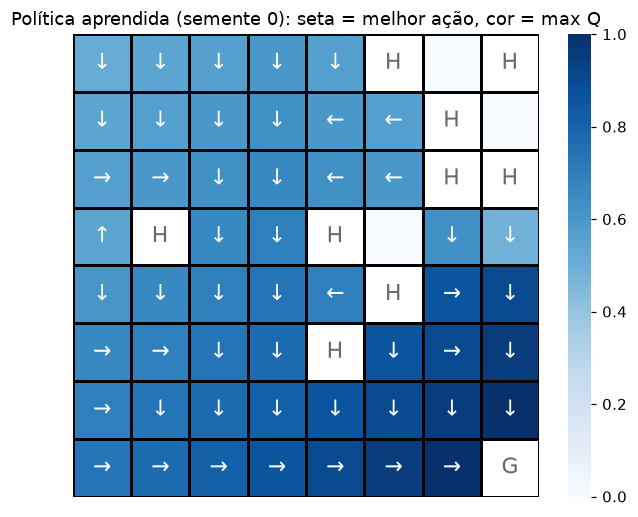
\includegraphics[width=0.4\textwidth]{exp0_politica.png}
  \caption{Política aprendida no 8x8 determinístico (semente 0). Cor: $\max_a Q(s,a)$; seta: melhor ação.}
  \label{fig:politica}
\end{figure}

A Tabela~\ref{tab:mapas} mostra a mesma configuração em dez mapas aleatórios. Todos chegaram a 100\% de sucesso, mas
o número de episódios até 90\% variou de 125 a 2008. Entre mapas, a média foi $667 \pm 599$ episódios. No mapa
fixo, variando só a semente do agente, foi $855 \pm 173$. Ou seja, \textbf{o mapa muda o resultado bem mais do que a
aleatoriedade do algoritmo}. Se cada execução gerasse um mapa novo, como no notebook original, não daria para saber
se uma diferença vem do hiperparâmetro ou do mapa. Por isso o mapa foi fixado nos demais experimentos.

\begin{table}[H]
\centering
\small
\caption{Configuração base em 10 mapas 8x8 aleatórios ($p = 0{,}9$), 3 sementes do agente por mapa.}
\label{tab:mapas}
\begin{tabular}{cccccccccccc}
\toprule
Mapa (semente) & 0 & 1 & 2 & 3 & 4 & 5 & 6 & 7 & 8 & 9 \\
\midrule
Buracos & 5 & 6 & 3 & 3 & 3 & 5 & 4 & 4 & 4 & 9 \\
Ep. até 90\% & 675 & 2008 & 183 & 133 & 125 & 1350 & 133 & 300 & 825 & 933 \\
Treino (últ. 500) & 0,90 & 0,87 & 0,93 & 0,96 & 0,97 & 0,87 & 0,91 & 0,93 & 0,91 & 0,90 \\
\bottomrule
\end{tabular}
\end{table}

\subsection*{Hiperparâmetros no FrozenLake 8x8 determinístico}

No mapa determinístico, \textbf{todas} as configurações chegaram a 100\% de sucesso guloso
(Tabela~\ref{tab:det}). Variando $\alpha$ e $\gamma$, o episódio em que o teste atinge 90\% foi o mesmo (855) em
todos os casos, e as curvas de teste se sobrepõem. O que mudou foi a exploração: $\varepsilon$ inicial $= 1{,}0$
convergiu mais cedo (710 episódios), e o $\varepsilon$ final definiu a recompensa de treino, de 0,975 com
$\varepsilon = 0{,}01$ a 0,714 com $\varepsilon = 0{,}3$ (Figura~\ref{fig:epsfinal}).

\begin{table}[H]
\centering
\small
\caption{FrozenLake 8x8 determinístico (média $\pm$ desvio padrão entre 5 sementes). Em todas as linhas, o sucesso
guloso final foi $1{,}000 \pm 0{,}000$.}
\label{tab:det}
\begin{tabular}{lcc}
\toprule
Configuração & Treino (últ. 500 ep.) & Ep. até 90\% \\
\midrule
$\alpha = 0{,}01$ & $0{,}920 \pm 0{,}036$ & 855 \\
$\alpha = 0{,}5$ (base) & $0{,}896 \pm 0{,}010$ & 855 \\
$\alpha = 0{,}9$  & $0{,}901 \pm 0{,}007$ & 855 \\
\midrule
$\gamma = 0{,}5$  & $0{,}902 \pm 0{,}004$ & 855 \\
$\gamma = 0{,}99$ & $0{,}908 \pm 0{,}021$ & 855 \\
\midrule
$\varepsilon$ inicial $= 0{,}1$ (constante) & $0{,}940 \pm 0{,}016$ & 845 \\
$\varepsilon$ inicial $= 1{,}0$ & $0{,}888 \pm 0{,}006$ & 710 \\
\midrule
$\varepsilon$ final $= 0{,}01$ & $0{,}975 \pm 0{,}007$ & 855 \\
$\varepsilon$ final $= 0{,}3$  & $0{,}714 \pm 0{,}021$ & 840 \\
\bottomrule
\end{tabular}
\end{table}

\begin{figure}[H]
  \centering
  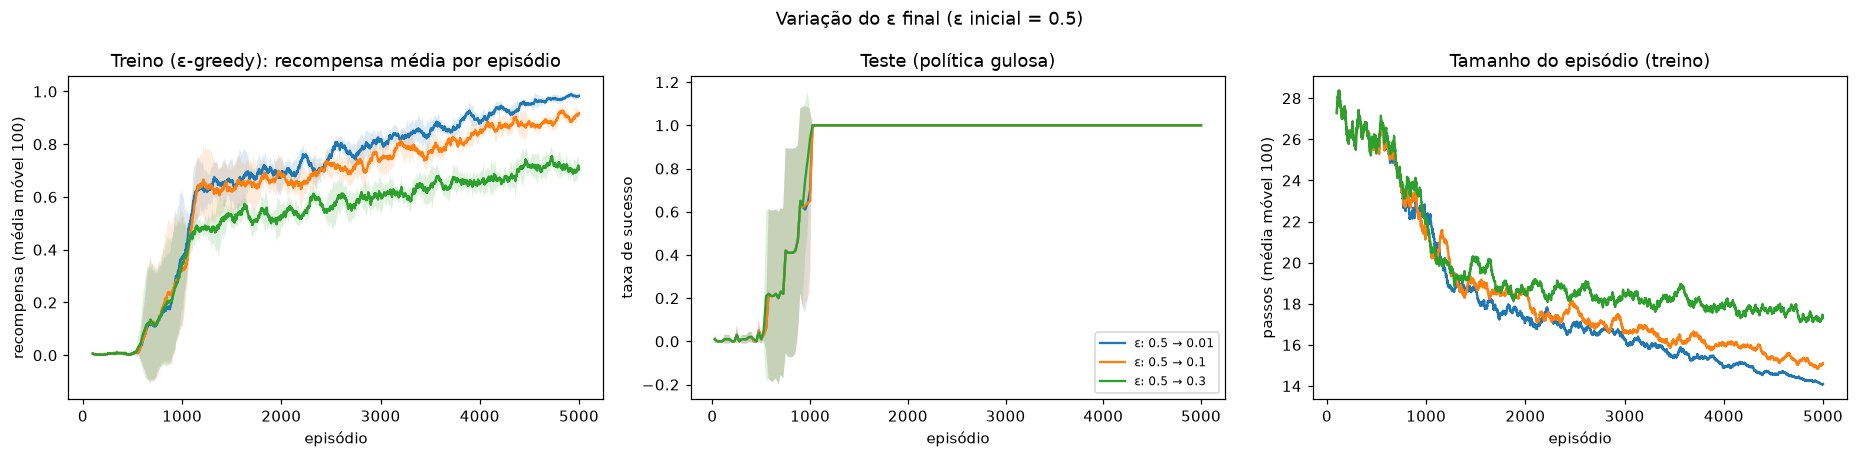
\includegraphics[width=0.85\textwidth]{exp2_epsilon_final.png}
  \caption{Variação do $\varepsilon$ final no 8x8 determinístico: o teste guloso é igual nos três casos; a recompensa
    de treino e o tamanho dos episódios, não.}
  \label{fig:epsfinal}
\end{figure}

\subsection*{Hiperparâmetros no FrozenLake 4x4 escorregadio}

No gelo escorregadio, os hiperparâmetros passaram a mudar a política final (Tabela~\ref{tab:esc} e
Figura~\ref{fig:esc-alpha}). Lembrando que o máximo possível é 0,744:

\begin{table}[H]
\centering
\small
\caption{FrozenLake 4x4 escorregadio (média $\pm$ desvio padrão entre 5 sementes). ``Ep. até 70\%'' é a média entre
as sementes que atingiram o limiar, entre parênteses.}
\label{tab:esc}
\begin{tabular}{lccc}
\toprule
Configuração & Sucesso guloso final & Treino (últ. 500 ep.) & Ep. até 70\% \\
\midrule
$\alpha = 0{,}01$ & $0{,}229 \pm 0{,}198$ & $0{,}145 \pm 0{,}091$ & 4075 (1/5) \\
$\alpha = 0{,}1$  & $\mathbf{0{,}544 \pm 0{,}138}$ & $0{,}308 \pm 0{,}016$ & 825 (5/5) \\
$\alpha = 0{,}5$ (base) & $0{,}400 \pm 0{,}241$ & $0{,}194 \pm 0{,}022$ & 535 (5/5) \\
$\alpha = 0{,}9$  & $0{,}272 \pm 0{,}246$ & $0{,}130 \pm 0{,}012$ & 2085 (5/5) \\
\midrule
$\gamma = 0{,}5$  & $0{,}128 \pm 0{,}054$ & $0{,}054 \pm 0{,}010$ & 3800 (1/5) \\
$\gamma = 0{,}9$  & $0{,}418 \pm 0{,}229$ & $0{,}170 \pm 0{,}012$ & 960 (5/5) \\
$\gamma = 0{,}99$ & $0{,}444 \pm 0{,}229$ & $0{,}232 \pm 0{,}017$ & 510 (5/5) \\
\midrule
$\varepsilon$ final $= 0{,}01$ & $\mathbf{0{,}665 \pm 0{,}106}$ & $0{,}389 \pm 0{,}036$ & 425 (5/5) \\
$\varepsilon$ final $= 0{,}3$  & $0{,}472 \pm 0{,}182$ & $0{,}078 \pm 0{,}010$ & 695 (5/5) \\
\bottomrule
\end{tabular}
\end{table}

\begin{figure}[H]
  \centering
  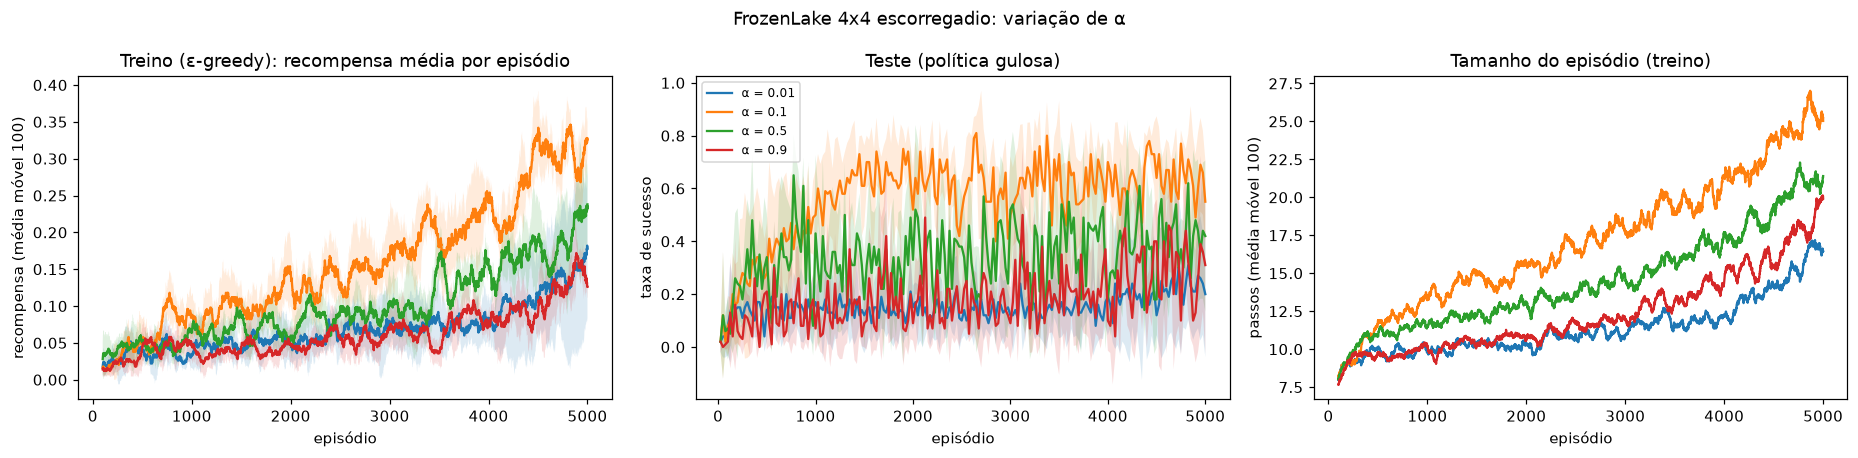
\includegraphics[width=0.85\textwidth]{exp2_escorregadio_alpha.png}
  \caption{Variação de $\alpha$ no 4x4 escorregadio.}
  \label{fig:esc-alpha}
\end{figure}

\subsection*{Tamanho do mapa e gelo escorregadio}

\begin{table}[H]
\centering
\small
\caption{Variações do FrozenLake (configuração base, salvo indicação).}
\label{tab:fl}
\begin{tabular}{lccc}
\toprule
Ambiente & Sucesso guloso final & Treino (últ. 500 ep.) & Ep. até 70\% \\
\midrule
4x4 determinístico & $1{,}000 \pm 0{,}000$ & $0{,}873 \pm 0{,}019$ & 165 (5/5) \\
4x4 escorregadio   & $0{,}400 \pm 0{,}241$ & $0{,}194 \pm 0{,}022$ & 535 (5/5) \\
8x8 determinístico & $1{,}000 \pm 0{,}000$ & $0{,}896 \pm 0{,}010$ & 855 (5/5) \\
8x8 escorregadio   & $0{,}390 \pm 0{,}115$ & $0{,}289 \pm 0{,}050$ & 1475 (5/5) \\
8x8 escorregadio, 20000 ep. & $0{,}412 \pm 0{,}145$ & $0{,}294 \pm 0{,}015$ & 1840 (5/5) \\
8x8 escorregadio, 20000 ep., $\alpha = 0{,}1$ & $\mathbf{0{,}694 \pm 0{,}196}$ & $0{,}523 \pm 0{,}013$ & 1890 (5/5) \\
\bottomrule
\end{tabular}
\end{table}

O mapa maior demorou mais para convergir (165 contra 855 episódios no determinístico). O gelo escorregadio derrubou o
desempenho nos dois tamanhos. No 8x8 escorregadio, \textbf{treinar 4 vezes mais com $\alpha = 0{,}5$ quase não
mudou o resultado} (0,390 para 0,412). Com $\alpha = 0{,}1$ e o mesmo número de episódios, o sucesso subiu para
0,694 (Figura~\ref{fig:20k}).

\begin{figure}[H]
  \centering
  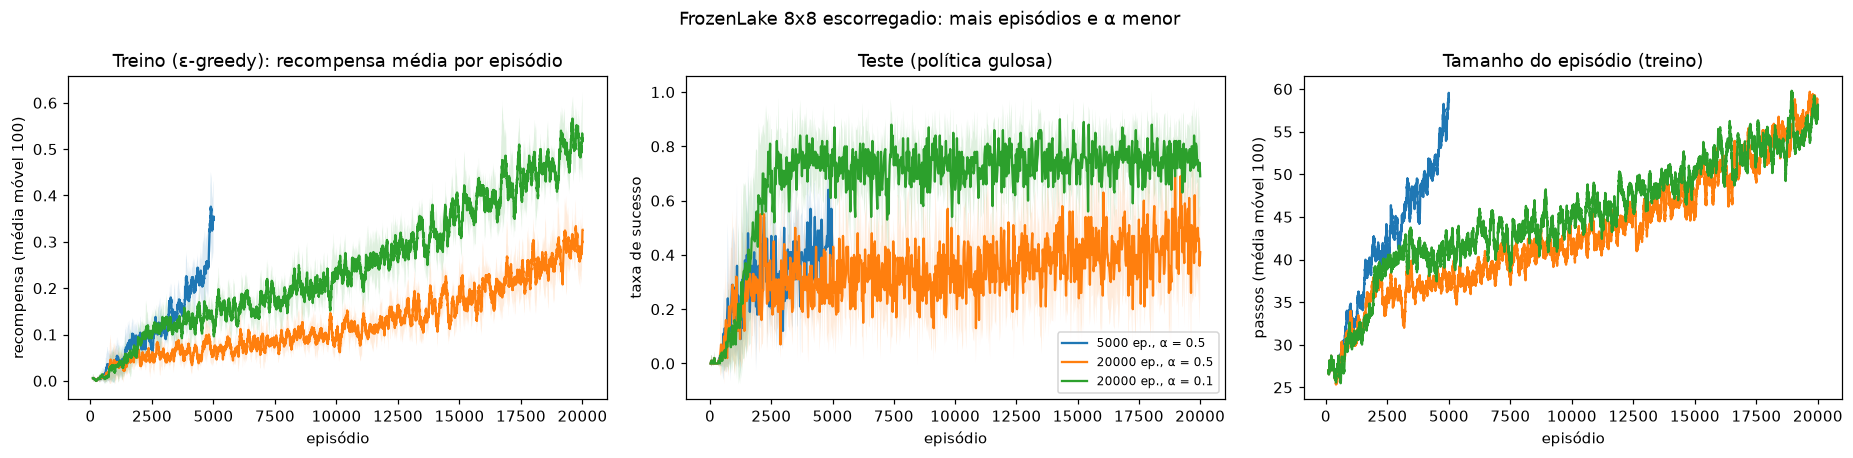
\includegraphics[width=0.85\textwidth]{exp3_escorregadio_20k.png}
  \caption{8x8 escorregadio: 5000 e 20000 episódios com $\alpha = 0{,}5$, e 20000 episódios com $\alpha = 0{,}1$.}
  \label{fig:20k}
\end{figure}

\subsection*{CliffWalking e Taxi}

\begin{table}[H]
\centering
\small
\caption{Outros ambientes, configuração base (retorno = soma das recompensas do episódio).}
\label{tab:outros}
\begin{tabular}{lccc}
\toprule
Ambiente & Retorno guloso final & Retorno de treino (últ. 500 ep.) & Ep. até o ótimo \\
\midrule
CliffWalking-v1 & $-13{,}00 \pm 0{,}00$ & $-62{,}77 \pm 3{,}24$ & 35 (5/5) \\
Taxi-v4 & $7{,}90 \pm 0{,}07$ & $1{,}07 \pm 0{,}17$ & 715 (5/5) \\
\bottomrule
\end{tabular}
\end{table}

No CliffWalking, a política gulosa encontrou o retorno ótimo ($-13$) muito cedo, em torno do episódio 35, e o manteve
até o fim (Figura~\ref{fig:cliff}). A recompensa de treino, no entanto, ficou em $-62{,}8$ nos últimos 500 episódios.
A política aprendida segue a linha logo acima do penhasco (Figura~\ref{fig:cliff-politica}). No Taxi, o agente chegou
a um retorno guloso de 7,90, perto do ótimo médio de 8,46, com o teste passando de 8 por volta do episódio 715.

\begin{figure}[H]
  \centering
  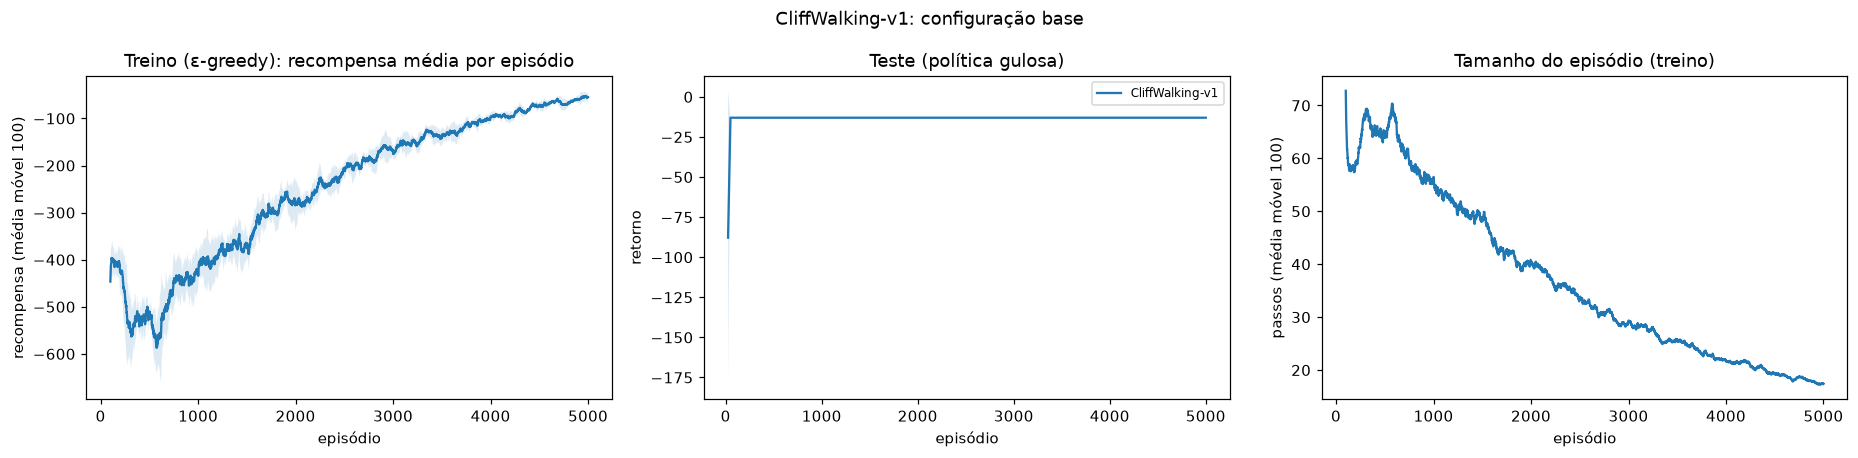
\includegraphics[width=0.85\textwidth]{exp4_cliffwalking.png}
  \caption{CliffWalking-v1: o teste guloso atinge $-13$ logo no início, mas o retorno de treino continua bem menor.}
  \label{fig:cliff}
\end{figure}

\begin{figure}[H]
  \centering
  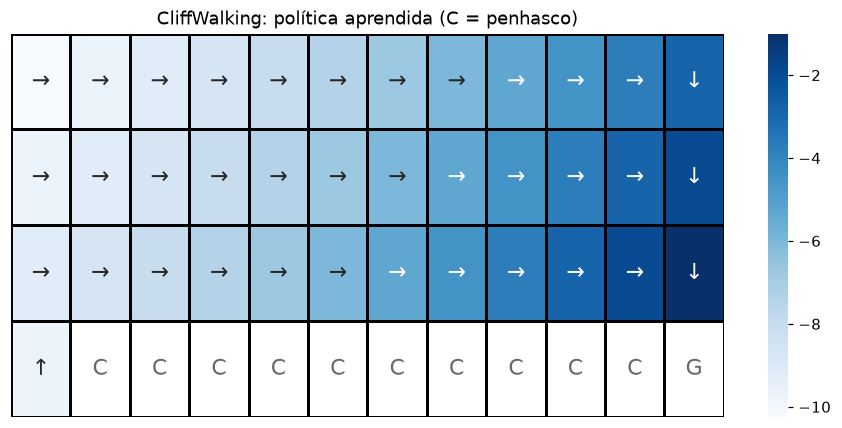
\includegraphics[width=0.55\textwidth]{exp4_cliff_politica.png}
  \caption{Política aprendida no CliffWalking (C = penhasco, G = objetivo).}
  \label{fig:cliff-politica}
\end{figure}

\subsection*{Análise qualitativa}

Em todos os FrozenLake há um período inicial com recompensa zero, até o agente achar o objetivo pela primeira vez;
depois o valor se propaga para trás e o teste guloso sobe em degraus. Com $\varepsilon$ final $= 0{,}3$ houve
exploração excessiva: o agente já sabia o caminho, mas continuou caindo em buracos no treino. No gelo escorregadio com
$\alpha$ alto, as curvas de teste oscilam muito e o desvio entre sementes chega a $\pm 0{,}24$, sinal de que a
Q-table não se estabiliza. Já os episódios ficam mais longos ao longo do treino, porque a política passa a contornar
os buracos em vez de arriscar o caminho mais curto.

\section{Discussão}

\textbf{H1 foi confirmada.} No mapa determinístico, com recompensas sempre $\geq 0$, qualquer $\alpha > 0$ e
$\gamma > 0$ tornam positivos os valores Q das ações que levam ao objetivo, e a política gulosa só depende de quais
valores são positivos. Como as sementes também eram as mesmas, o agente tomou as mesmas decisões até convergir em todas
as variações de $\alpha$ e $\gamma$, o que explica os 855 episódios repetidos e as curvas de teste sobrepostas. Nesse cenário, só a exploração mudou a
velocidade: com $\varepsilon$ inicial $= 1{,}0$, o agente cobre o mapa mais rápido e acha o objetivo mais cedo.

\textbf{H2 foi confirmada.} No gelo escorregadio, $\alpha$ precisa ser pequeno o bastante para fazer a média dos
resultados aleatórios, mas não tão pequeno que o aprendizado não ande. O melhor valor foi $\alpha = 0{,}1$; com
$\alpha = 0{,}01$ o aprendizado foi lento demais para 5000 episódios, e com 0,5 e 0,9 a Q-table oscilou. Isso bate
com a teoria: a convergência do Q-learning para $Q^*$ pede que a taxa de aprendizado diminua ao longo do tempo. Com
$\alpha$ constante e alto, os valores ficam reagindo a cada escorregão, e a política final é um retrato ruidoso da
tabela. Por isso treinar quatro vezes mais com $\alpha = 0{,}5$ não ajudou, e reduzir $\alpha$ ajudou.

\textbf{H3 foi confirmada.} Com $\gamma = 0{,}5$, o valor do objetivo a $k$ passos vale $0{,}5^k$. No 4x4
escorregadio, onde o agente precisa de vários passos (e de desvios) para chegar, esse valor fica pequeno demais para
distinguir as ações, e o sucesso caiu para 0,13. Entre 0,9 e 0,99, as diferenças ficaram dentro do desvio padrão.

\textbf{H4 foi confirmada}, com uma ressalva. Um $\varepsilon$ final maior piorou a recompensa de treino em todos os
casos. Mas a política gulosa final do 4x4 escorregadio foi melhor com $\varepsilon$ final $= 0{,}01$ (0,665) do que com
0,1 (0,400). Uma explicação é que, explorando menos no fim, o agente visita mais o caminho que de fato usa e estima
melhor os valores Q dali; mas as diferenças estão dentro do desvio padrão.

\textbf{H5 foi confirmada.} No CliffWalking, o Q-learning aprende o valor da política gulosa (pelo
$\max_{a'} Q(s',a')$) e não o da política $\varepsilon$-greedy que de fato executa. Ele por isso aprende o caminho
ótimo colado no penhasco, mas, durante o treino, os passos aleatórios ali custam $-100$. É o exemplo clássico de
Sutton e Barto: um método \emph{on-policy} como o SARSA aprenderia um caminho mais afastado do penhasco, com retorno
de treino melhor e política final pior.

\textbf{Limitações.} Foram só 5 sementes por configuração, e no gelo escorregadio várias diferenças ficaram
dentro do desvio padrão. Os hiperparâmetros foram variados um de cada vez, sem testar combinações, e em um mapa de cada
tamanho, embora o Experimento 1 mostre que o mapa influencia bastante. Além disso, o CliffWalking recebeu um limite de
200 passos que o ambiente original não tem.

\textbf{Melhorias possíveis:} taxa de aprendizado decrescente (por exemplo, $\alpha = 1/N(s,a)$, em que $N$ é o número
de visitas ao par); outras estratégias de exploração, como decaimento exponencial de $\varepsilon$, softmax ou
inicialização otimista da Q-table; mais sementes e mais mapas; e uma busca conjunta de hiperparâmetros.

\section{Conclusões}

O Q-learning resolveu todos os ambientes determinísticos testados (ótimo no FrozenLake e no CliffWalking, perto do
ótimo no Taxi), e neles os hiperparâmetros mudaram só a velocidade e a recompensa de treino, não a política final. No gelo escorregadio a situação mudou: o
resultado dependeu bastante de $\alpha$, $\gamma$ e $\varepsilon$, e a melhor configuração encontrada ($\alpha = 0{,}1$
com 20000 episódios no 8x8; $\varepsilon$ final $= 0{,}01$ no 4x4) ficou entre 78\% e 89\% do máximo possível.

As principais lições foram:
\begin{itemize}
  \item a recompensa de treino e o desempenho da política aprendida são medidas diferentes, e é preciso olhar as duas
    (CliffWalking e $\varepsilon$ final);
  \item em ambientes estocásticos, a taxa de aprendizado é decisiva, e treinar mais não compensa um $\alpha$ alto;
  \item para comparar configurações é preciso controlar a aleatoriedade (mapa fixo e várias sementes), porque o mapa
    sozinho mudou a velocidade de convergência em mais de 10 vezes.
\end{itemize}

Como próximos passos, ficam a comparação com o SARSA no CliffWalking e o uso de $\alpha$ decrescente no gelo
escorregadio.

\end{document}
